%% 
%\documentclass[a4paper,fleqn,longmktitle]{cas-sc}
\documentclass[a4paper,fleqn]{cas-sc}
\usepackage[numbers]{natbib}

%%%Author macros
\def\tsc#1{\csdef{#1}{\textsc{\lowercase{#1}}\xspace}}
\tsc{WGM}
\tsc{QE}
\tsc{EP}
\tsc{PMS}
\tsc{BEC}
\tsc{DE}
%%%
\usepackage{braket}
\usepackage{bm}

\begin{document}
	\let\WriteBookmarks\relax
	\def\floatpagepagefraction{1}
	\def\textpagefraction{.001}
	\shorttitle{Optimization of wide-band quasi-omnidirectional 1-D photonic structures}
	\shortauthors{V. Castillo-Gallardo et~al.}
	
	\title [mode = title]{Suplementary information: Optimization of wide-band quasi-omnidirectional 1-D photonic structures}                      	
	\author[1,2,3]{V. Castillo-Gallardo}
	\cormark[1]
	\ead{ing.victorcg@gmail.com}
	\credit{Conceptualization, Software $\&$ Investigation, synthesis $\&$ characterization, Writing}
	\address[1]{Centro de Investigaci\'{o}n en Ingenier\'{i}a y
		Ciencias Aplicadas, Universidad del Estado de Morelos, Av.
		Universidad 1001, Col. Chamilpa, Cuernavaca, Morelos 62209,
		M\'{e}xico.}
	
	\author[1,2,3]{Luis Eduardo Puente-D\'{i}az}
	\ead{fmatpuente@gmail.com}
	\credit{Software $\&$ Investigation}
	\address[2]{Instituto de Ciencias F\'{i}sicas, Universidad
		Nacional Aut\'{o}noma de M\'{e}xico, Av. Universidad S/N,
		Col. Chamilpa, 62210 Cuernavaca, Morelos, M\'{e}xico.}
	\address[3]{Facultad de Ciencias F\'{i}sico Matem\'{a}ticas,
		Universidad Michoacana de San Nicol\'{a}s de Hidalgo, Av.
		Francisco J. Múgica S/N 58030, Morelia, Mich., M\'{e}xico.}
	
	\author[4]{D. Ariza-Flores}
	\ead{david1cool@gmail.com}
	\credit{Investigation, Writing - review $\&$ editing}
	\address[4]{CONACyT-Universidad Aut\'{o}noma de San Luis
		Potos\'{i}, Karakorum 1470, Lomas 4ta Secc, San Luis Potos\'{i},
		S.L.P., 78210, M\'{e}xico.}
	
	\author[3]{H\'{e}ctor P\'{e}rez-Aguilar}
	\ead{hiperezag@yahoo.com}
	\credit{Investigation and Supervision}
	
	\author[2]{W. Luis Moch\'{a}n}
	\cormark[2]
	\ead{mochan@fis.unam.mx}
	\credit{Conceptualization, Funding acquisition, Software $\&$ Investigation, Methodology, Supervision, Writing - review $\&$ editing}
	
	\author[1]{V Agarwal}
	\cormark[3]
	\fnmark[1]
	\ead{vagarwal@uaem.mx}
	\credit{Conceptualization, Funding acquisition, Investigation, Methodology, Supervision, Writing - review $\&$ editing}
	
	\cortext[cor1]{Corresponding author}
	\cortext[cor2]{Corresponding author}
	\cortext[cor3]{Principal corresponding author}
	\fntext[fn1]{On sabatical leave at ICF-UNAM from CIICAP-UAEM}
	
	\begin{abstract}
		Porous silicon is a very versatile material for developing optical
		devices based on multilayered structures, since high and low porosity layers
		can be synthesized by a simple electrochemical technique. In the present work, we design
		mirrors using \textit{chirped}-type structures and by stacking
		appropriately tuned sub-mirrors, and we optimize the design parameters
		to maximize the
		optical reflectance $\braket{R}$ averaged within a wide
		spectral range  covering the visible and near infrared regions, and
		within a wide angular range using low refractive index contrast. The chirped structures are found to be
		more suitable for the visible range,
		while stacked sub-mirrors are found to be better for the NIR
		region. We design, fabricate and characterize
		some of the optimized omnidirectional mirrors with less
		than 100 pairs of layers. We obtained structures with a wider
		omnidirectional spectral region (almost 1.4 times) and low refractive index contrast ratio than those previously
		reported.
	\end{abstract}
	
	\begin{keywords}
		Optimized reflectance \sep Omnidirectional structures \sep 
		Chirped structures \sep Stacked Bragg mirror structures
	\end{keywords}
\maketitle

\section{Chirped structure}
As expected, with an increase in the porosity contrast of the periods, the thickness 
of the structure decreases and the average reflectance increases. For 
example, one could have structures with a thickness of approx. 10 $\mu$m with the 
average reflectance greater than 90$\%$ for a wide spectral range, i.e., 350-1400nm, 
as shown in first block of table \ref{tab:tableA}. This block represents structures 
with porosities of $p_l=0.30$ and $p_h=0.76$. The second block manifiest the 
optimized parameters for structures with porosities of $p_l=0.42$ and $p_h=0.76$.

The mapping of the calculated reflectance of the structures designed with the 
optimized parameters is shown in Fig. \ref{Fig2}. Here it is observed that all of 
them have a ODB in the NIR region of the electromagnetic spectrum, i. e.,  
structures designed from functions $f_{1}$ and $f_{3}$ with a porosity contrast of 
$30/76\%$ have the highest ODB localized from 970 to 1370 nm, these are shown in 
panels (a) and (c). 	
	
\begin{table}[!ht]
  \centering
  \label{tab:tableA}
  \addtolength{\tabcolsep}{-2pt}
    \begin{tabular}{rrrrrrrrrr}
      Class&$\alpha$&$\beta$&A&$\lambda_{min}(nm)$&$N_{p}$&$d(\mu\text{m})$       &ODW(nm)&ODC (nm)&$\braket{R}(\%)$\\
      \hline
      \hline
      $f_{1}$     &0.55    &---      &---     &400&30   &9.2    
      &380    &1170    &92\\
      $f_{2}$     &0.22    &4.30     &---     &430&66   &17.8
      &280    &1190    &93\\
      $f_{3}$     & 1.15   &0.56   & 0.09    &400&30   & 10.5
      & 400& 1150& 91\\
      \hline
      $f_{1}$     & 0.35    & ---  & ---     &400&101    & 35.7
      &350& 1195& 91\\
      $f_{2}$     &0.45    &1.23     &0.5  &410  &105   &9.8     &280    &1170    &89\\
      $f_{3}$     &1.01    &0.50     &0.10  &350  &50   &16.4    &350    &1195    &90\\
    \end{tabular}
    %\caption{ Design parameters obtained after the optimization of functions for maximum average reflectance and minimum thickness}
  \caption{Optimized parameters $\alpha$, $\beta$, $A$ and $N_p$ yielding the highest
    reflectance $\braket{R}$ averaged over the spectral range $350-1400$ nm and
    the angular range $0-90^\circ$ for the profile classes $f_1$, $f_2$ and
    $f_3$. Structures have porosities of $p_l=0.30$ and $p_h=0.76$ (first block), and $p_l=0.42$ and $p_l=0.76$ (second block). We include the thickness $d$ of the structure, the omnidirectional spectral width (ODW) and the central wavelength (ODC).}
\end{table}

\begin{figure}[!ht]
	\begin{center}
		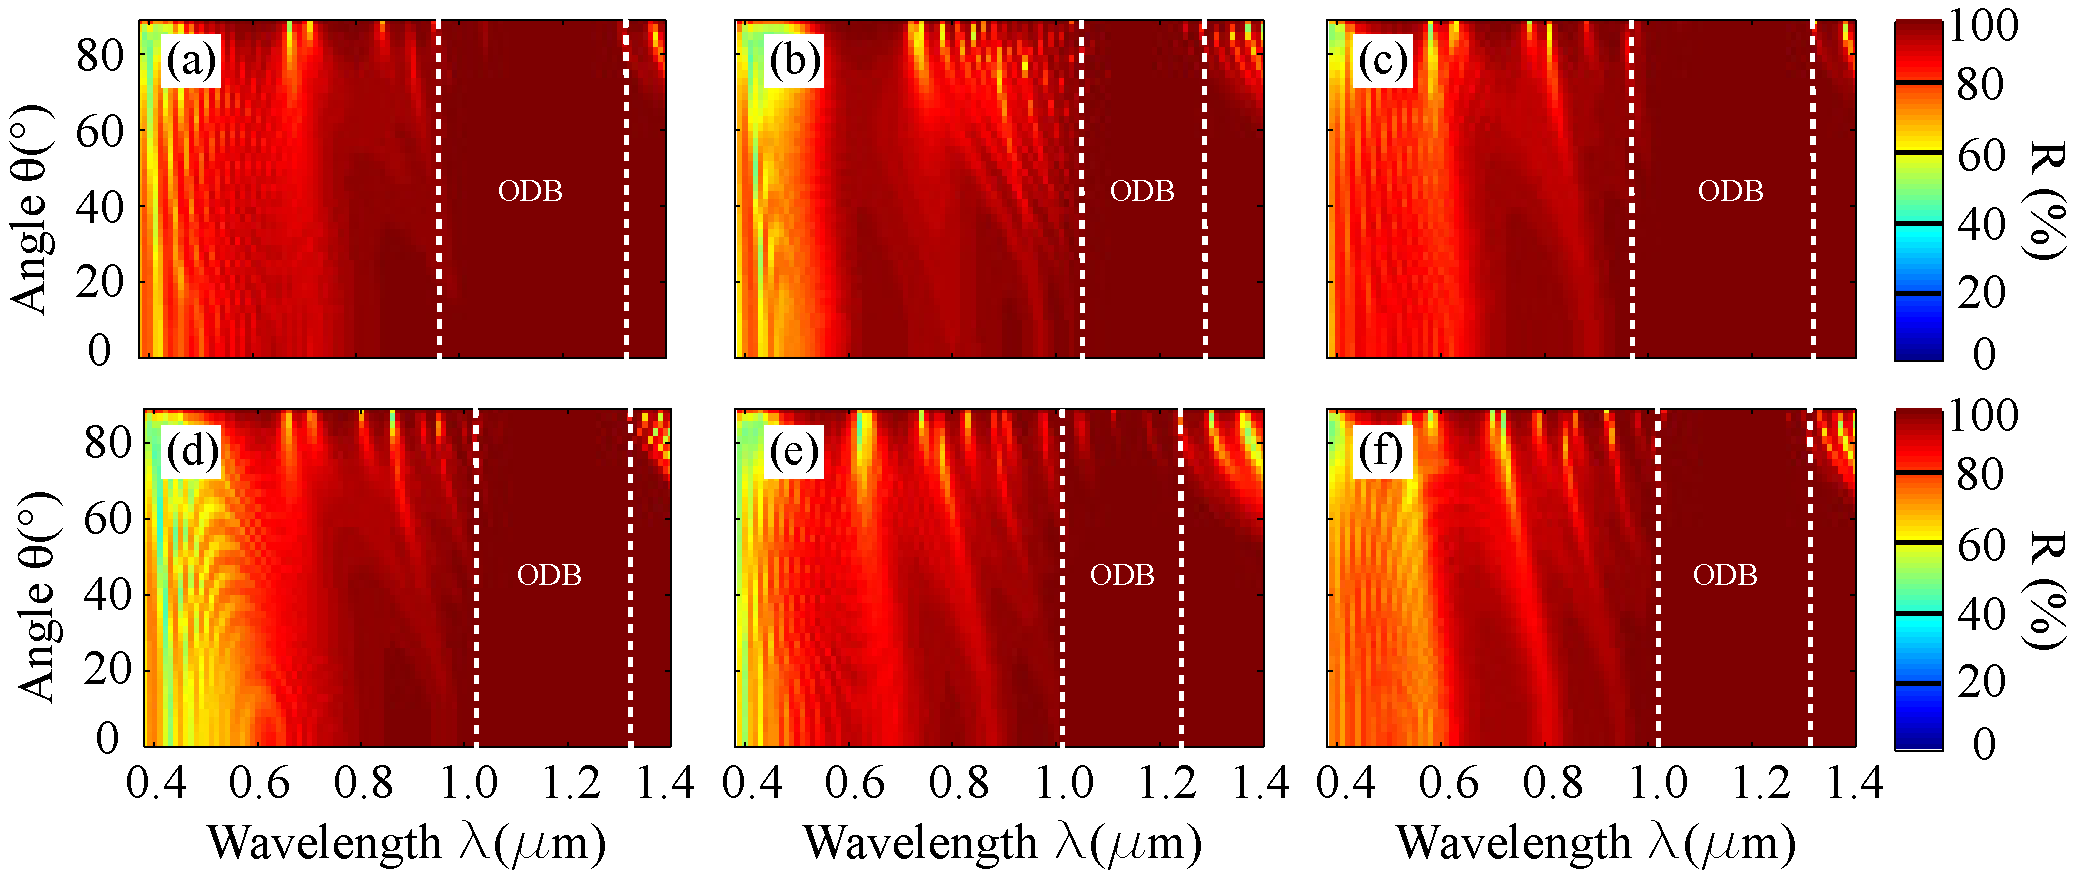
\includegraphics[width=\textwidth]
		{FigureS1.pdf}
	\end{center}
	\caption{Calculated reflectance of the structures designed with the optimized parameters of $f_{1}$ (left), $f_{2}$ (center) and $f_{3}$ (right) and with the porosity contrasts of $30/76\%$ (upper panels) and $42/76\%$ (lower panels). The dotted lines limit the area of the ODB.}
	\label{Fig2}
\end{figure}

\newpage

\section{Stacked sub-mirrors structure}

Additionally, the T$r|\text{M}|$ and R$(\lambda,\theta)$ were calculated for light with TE 
polarization and 45${{}^\circ}$ of incidence. In Fig. 3d it is shown that by using 
mirrors that have 6 periods and designed to reflect at wavelengths greater than 1000 
nm, they also reflect in a certain region of the visible spectrum. Then, to 
reinforce the reflection of the electromagnetic waves in the visible, it is enough 
to place a smaller number of periods. This is another reason for the increasing 
number of periods in the 400 to 800 nm region. 
\begin{figure}[!ht]
	\begin{center}
		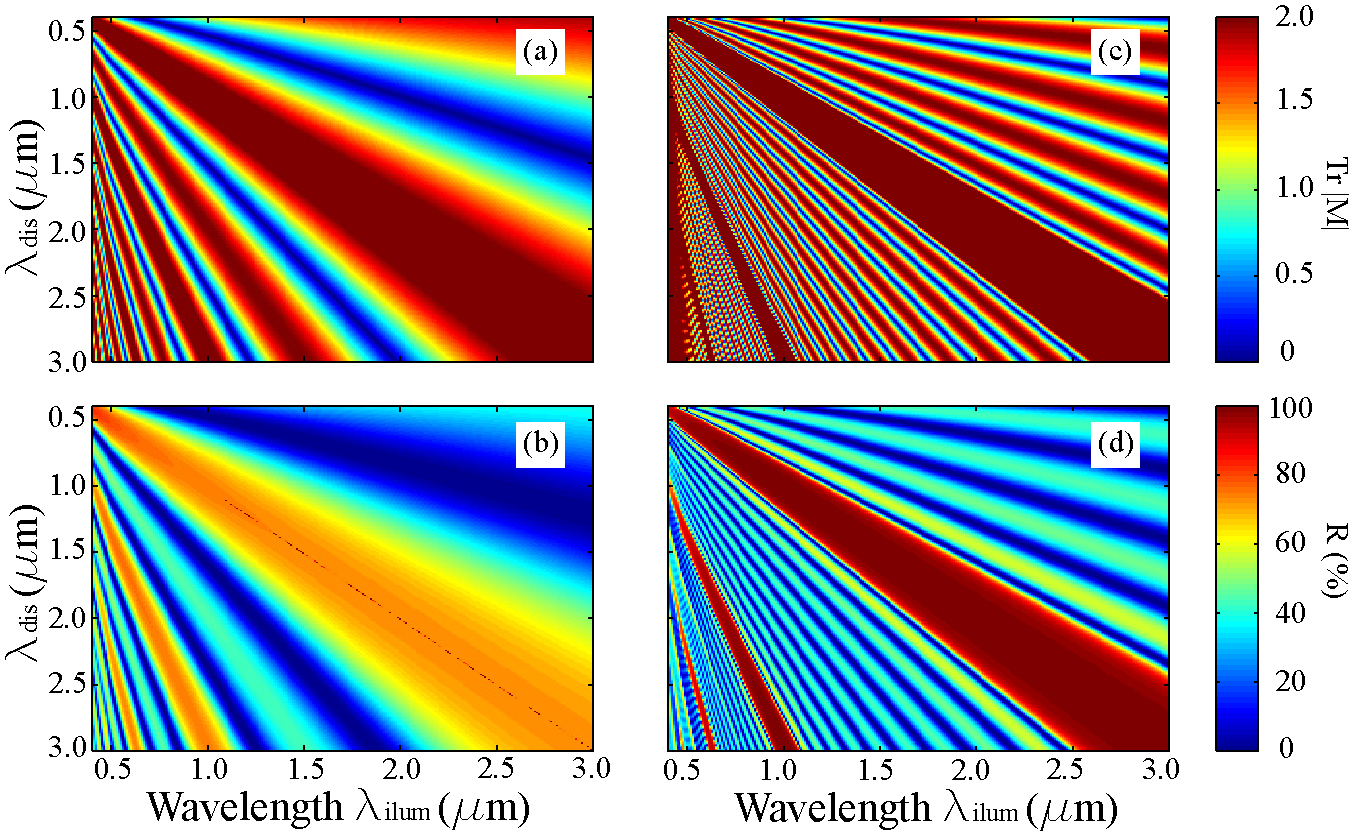
\includegraphics[width=\textwidth]
		{FigureS2.pdf}
	\end{center}
	\caption{Calculated transfer matrix trace and reflectance of individual mirrors using ((a) and (b)) one period  and ((c) and (d)) six periods, respectively. Each mirror was tuned to a wavelength between 400 and 3000 nm. The calculations were made in the visible and NIR region and at 45${{}^\circ}$ of incidence.}
	\label{Fig3}
\end{figure}
%\newpage

It is common to imagine that the stacking of the sub-mirrors in such a way that
the ODB of the second mirror begins at the edge of the ODB of the first mirror, the 
third ODB that begins at the edge of the ODB of the second mirror, and so on until 
the desired interval is completed. With this configuration, the reflectance 
decreases at each intersection of the two ODBs. For example, in Figs. \ref{Fig4}(a) 
and \ref{Fig4}(b) show the calculated R$(\lambda, \theta)$ for the structures formed 
by sub-mirrors that have one and six periods, respectively, using non-polarized 
light.  The R$_{Ave}(\lambda, \theta)$ was maximized through the percentage of 
overlap of the ODBs of two consecutive sub-mirrors.  
The 
calculated R$(\lambda, \theta)$ for the structures designed with 4 periods for each 
sub-mirror and using the pattern described in the main article are shown in Figs. 
\ref{Fig4}(c) and \ref{Fig4}(d) of this document, respectively. Here the overlap of 
the two consecutive ODBs was optimized, being $72\%$ for the first case and $78\%$ 
for the last. The calculations reveal the quasi-ODB of the structures.

\begin{figure}[!ht]
	\begin{center}
		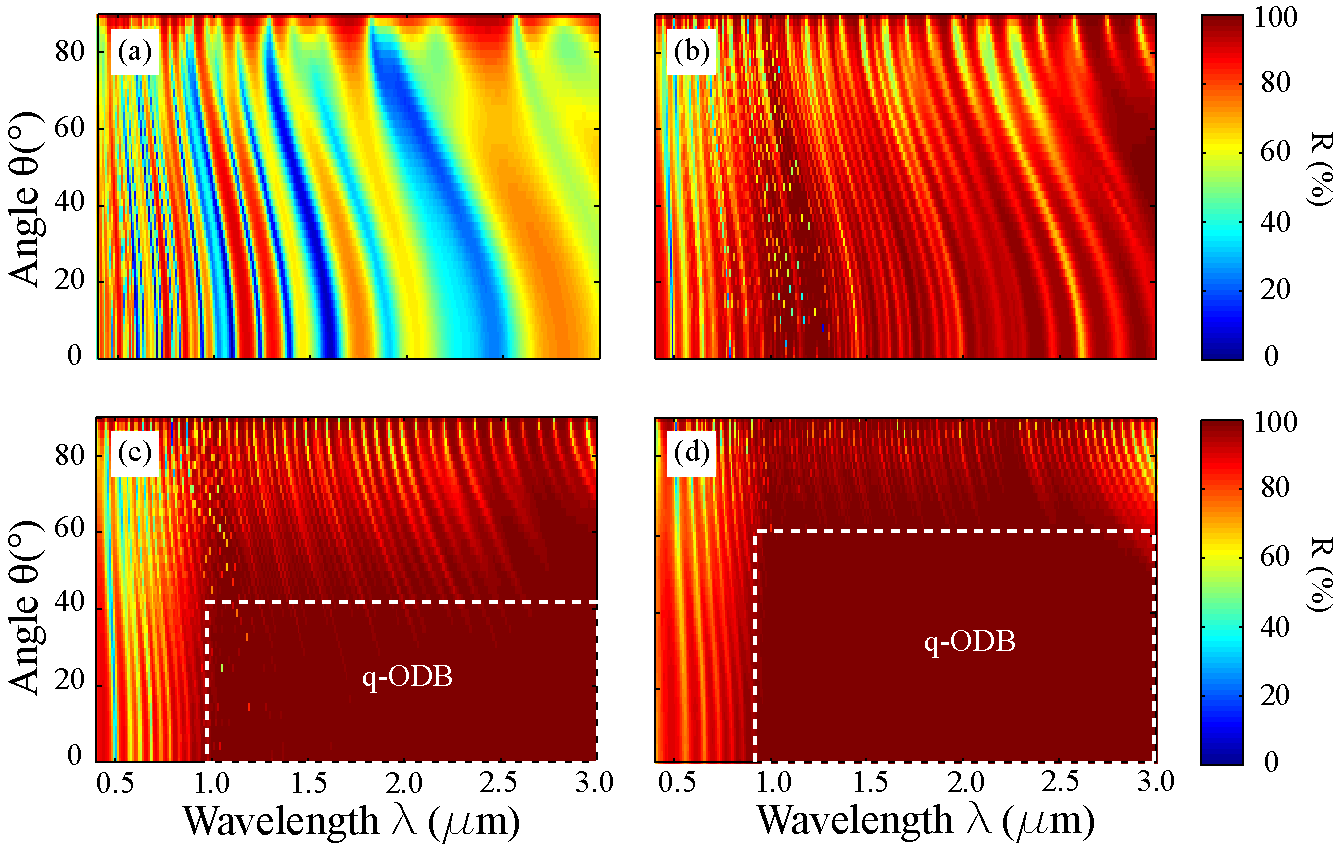
\includegraphics[width=\textwidth]
		{FigureS3.pdf}
	\end{center}
	\caption{Reflectance calculated for structures designed through the stacking of 
		sub-mirrors analyzing the overlap of the ODB and the number of periods in 
		each case. 
		Case I: there is no overlap of the ODBs and each 
		sub-mirror has (a) one period and (b) six periods. Case II: optimized 
		overlap of consecutive ODBs and (c) each submirror has 4 periods with 
		$72\%$ overlap, and (d) proposed arrangement in the main article with 6 
		periods for $\lambda>800$ nm and $78\%$ overlap. The quasi-OD region is indicated by the dotted lines.
	}
	\label{Fig4}
\end{figure}

\end{document}
